\chapter{Metodologia}
  \section{Gerenciamento}
    \subsection{Estrutura Analítica do Projeto (EAP)}

      Tendo como objetivo a visão geral sobre as atividades que serão
      realizadas no decorrer do projeto, escolheu-se a EAP como forma
      de organização sistematizada das informações.

      A EAP consiste em uma organização das entregas
      a serem feitas em um formato de árvore, partindo de tarefas
      mais gerais para tarefas mais específicas \cite{pmbok2012}.

      Para a construção da EAP, foram levados em conta as diferentes
      entregas a serem realizadas dentro do ciclo de vida do projeto,
      assim como as áreas de atuação dentro da equipe. Além disso, é
      possível observar o alinhamento da EAP com as atividades previstas
      no cronograma e com os requisitos estabelecidos para o projeto.

      A figura \ref{fig:eap} é a representação gráfica da EAP do projeto.

      \begin{figure}[!htbp]
        \centering
        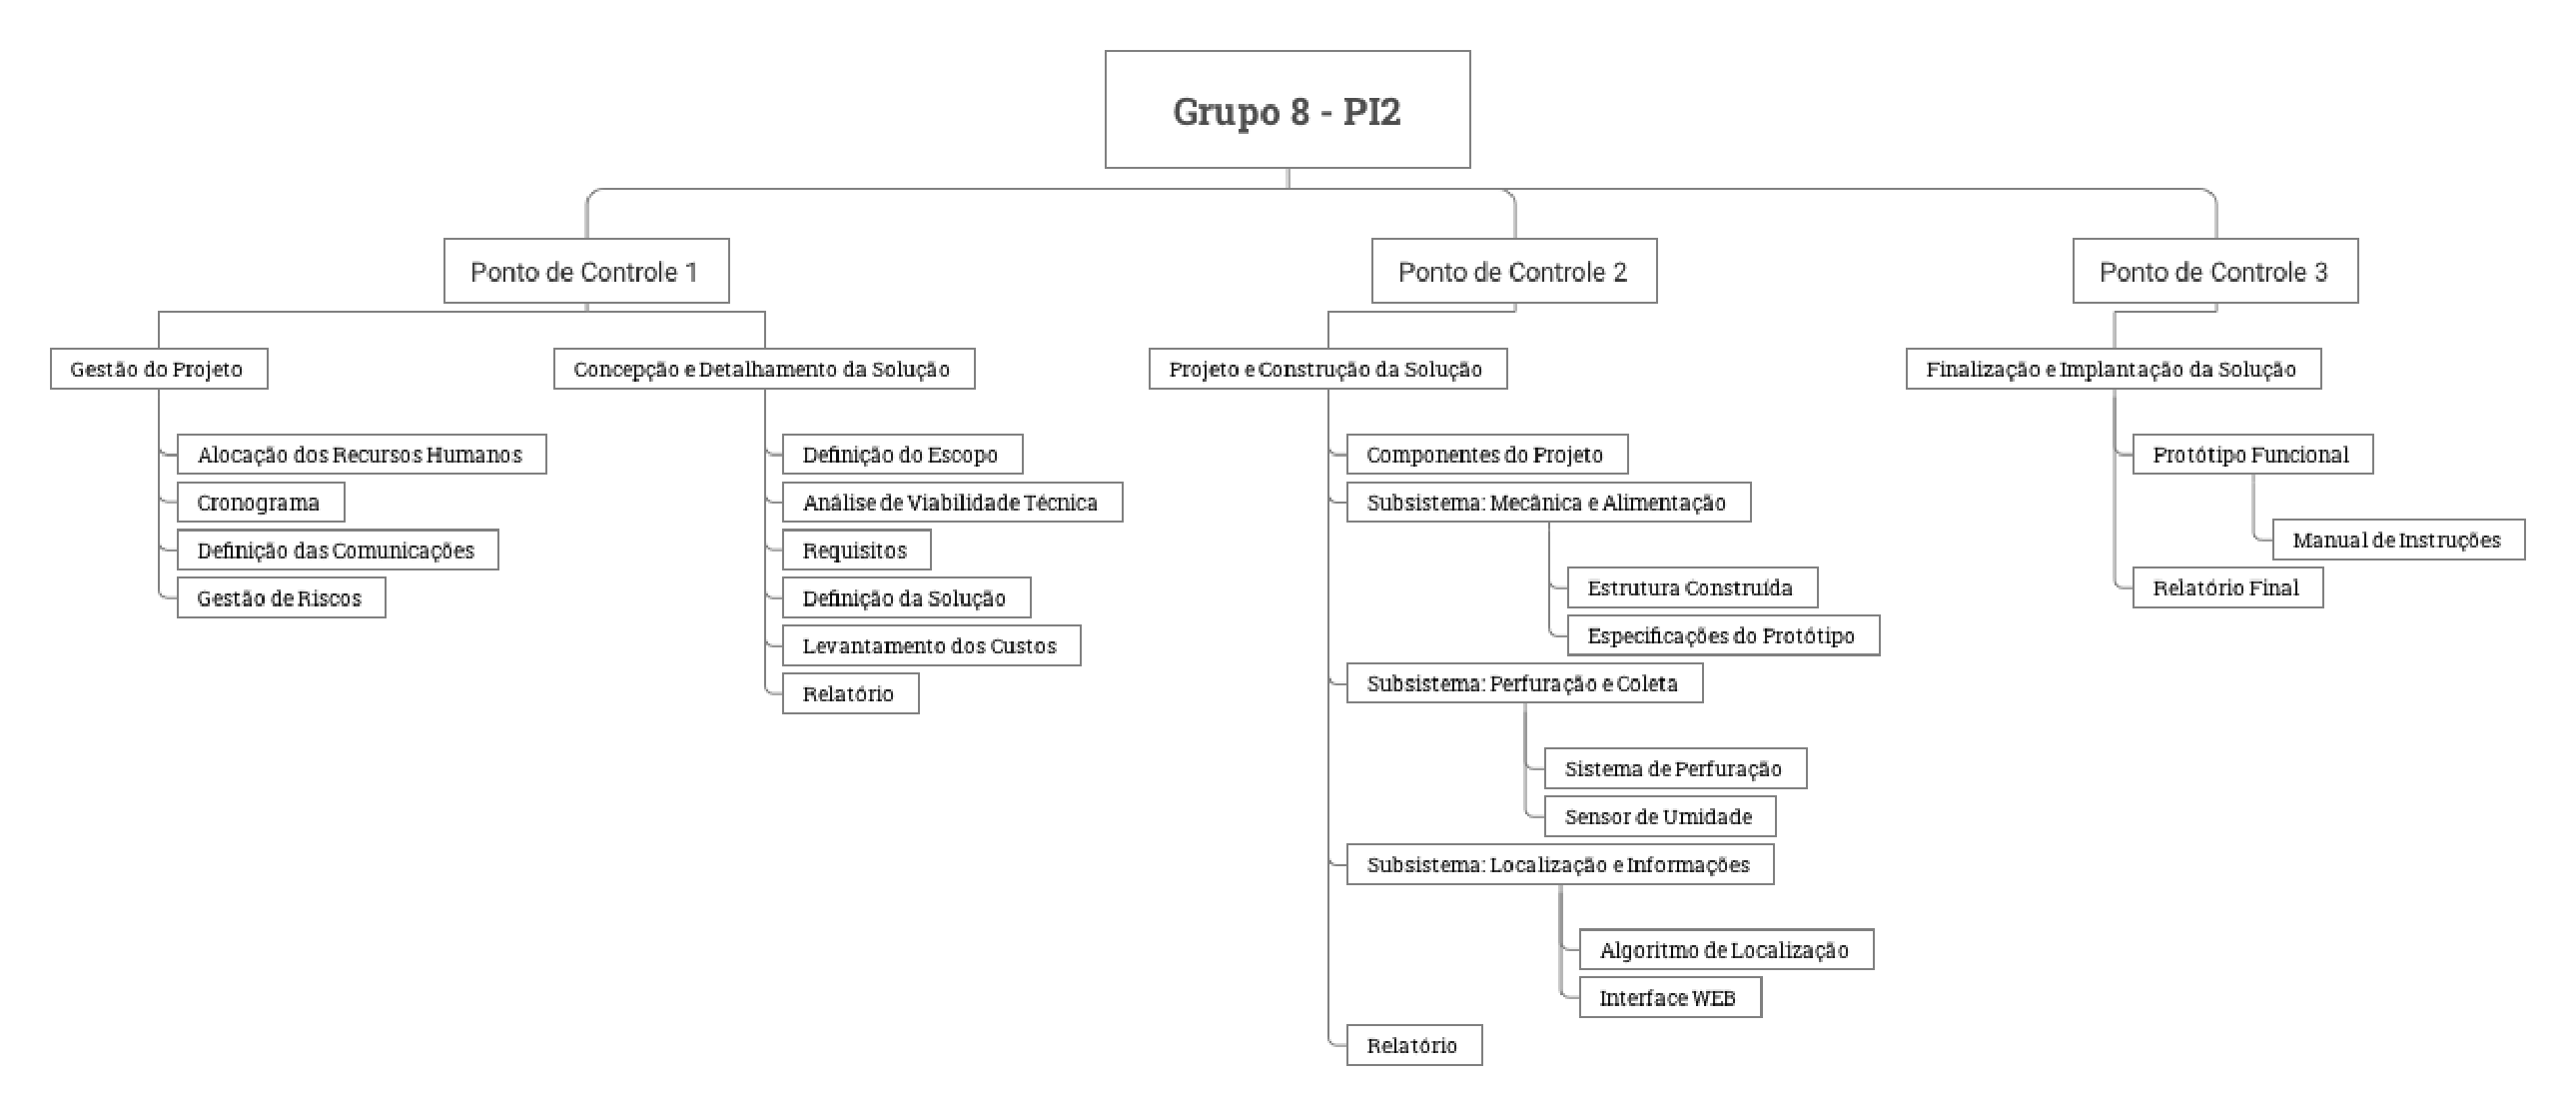
\includegraphics[width=\textwidth]{figuras/EAP.eps}
        \caption{Estrutura Analítica do Projeto. Fonte: autores.}
        \label{fig:eap}
      \end{figure}

      \vfill
      \pagebreak

    \subsection{Alocação dos Recursos Humanos}

      A equipe do projeto, formada por 15 (quinze) integrantes, foi
      subdivida em 3 (três) áreas de atuação, que são: "Mecânica e Alimentação", "Perfuração e Coleta" e "Localização e Informações".

      As áreas são supervisionadas e administradas por uma gestora geral, Jéssica Guimarães,
      e por um gestor da qualidade, Leonardo Cambraia.

      Cada uma das áreas citadas acimas é responsável pela análise de alternativas
      para a solução e a escolha de uma destas para ser aplicada no projeto.

      A figura \ref{fig:aloc} ilustra a estrutura de alocação de recursos humanos do
      projeto. A divisão dos integrantes foi feita levando em conta o
      interesse e conhecimento prévio individual nas áreas propostas.
      É importante salientar que toda a estrutura está sujeita a mudanças, sempre
      visando suprir as necessidades do projeto.

      \begin{figure}[!htbp]
        \centering
        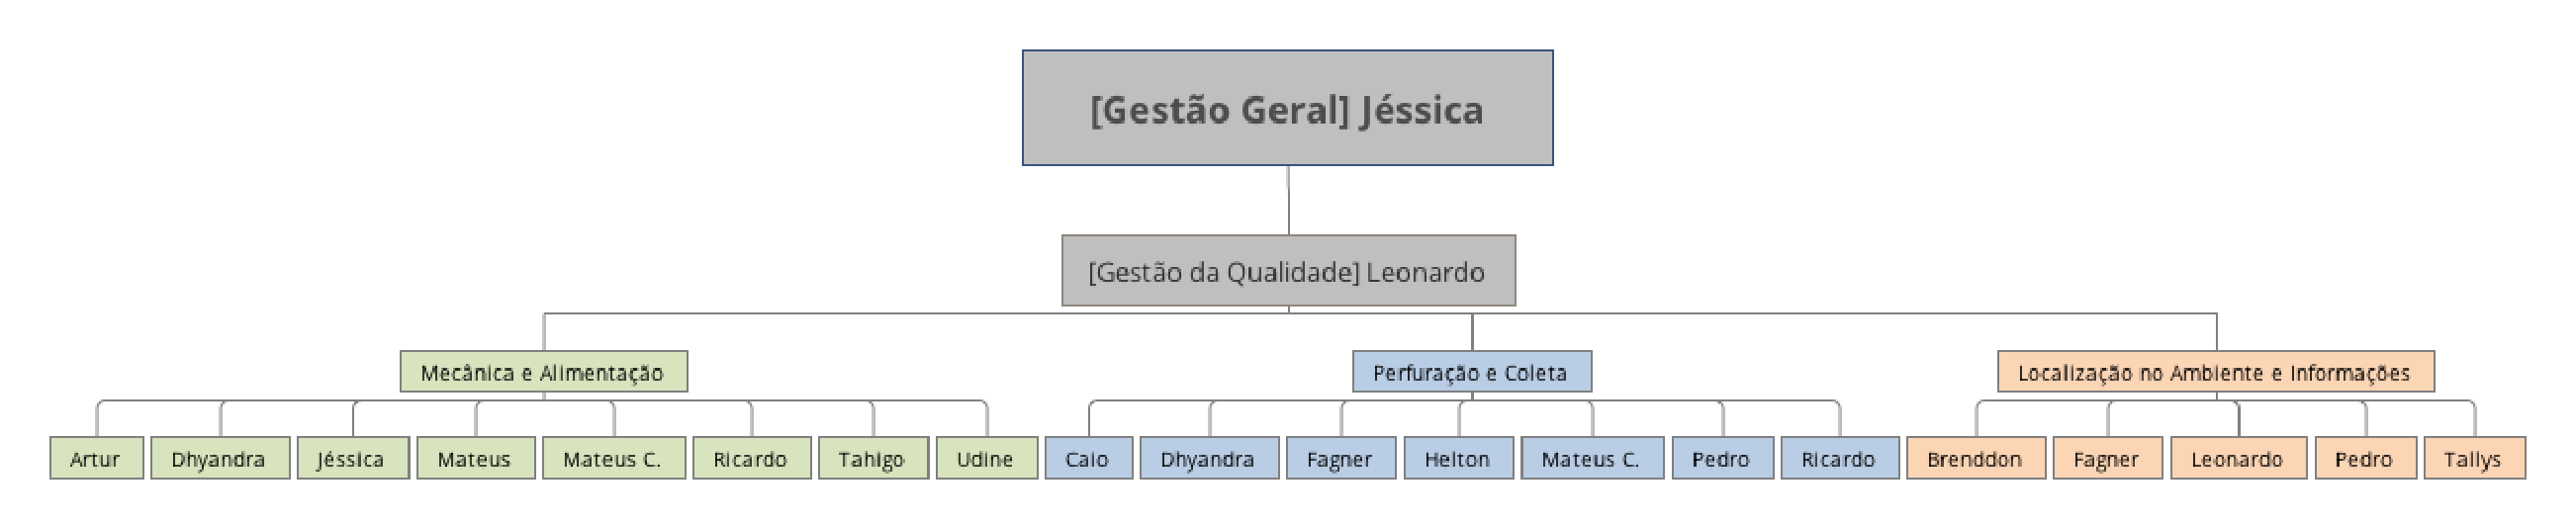
\includegraphics[width=\textwidth]{figuras/alocacao.eps}
        \caption{Alocação de recursos humanos. Fonte: autores.}
        \label{fig:aloc}
      \end{figure}

    \subsection{Comunicação}

      Para que qualquer projeto tenha sucesso é necessário o engajamento da equipe, sendo assim, é necessário uma comunicação eficaz entre os membros da equipe. A tabela \ref{tab:com} detalha os métodos de comunicação utilizados pela equipe.
      
      \begin{table}[!htbp]
      	\begin{center}
      		\caption{\label{tab:com}Métodos de comunicação. Fonte: autores.}
      		\begin{tabular}{|p{4cm}|p{4cm}|p{3cm}|p{3cm}|p{2cm}|}
      			\hline
      			\textbf{Objetivos} & \textbf{Ferramenta} & \textbf{Frequência} & \textbf{Horário} & \textbf{Local}\\\hline\hline
      			Acompanhamento das atividades & Kanban & Sob demanda & Horário da disciplina & FGA\\\hline
      			Avisos rápidos / Lembretes & Telegram & Sob demanda & N/A & N/A\\\hline
      			Decisões Técnicas/Planejamentos & Presencial & Duas vezes por semana & Horário da disciplina & FGA\\\hline
      			Desenvolvimento do projeto & Google Docs/ Google Hangouts/ Git / Github / Presencial & Sob demanda & Durante desenvolvimento do projeto & N/A\\\hline
      		\end{tabular}
      	\end{center}
      \end{table}

    \subsection{Tempo}

      Para a definição das atividades a serem realizadas durante o
      projeto utilizou-se como base os pacotes de trabalho estabelecidos
      na Estrutura Analítica do Projeto (EAP), onde os mesmos foram devidamente
      decompostos com base nos três grandes marcos do projeto referentes
      às entregas de Ponto de Controle 1, 2 e 3. Para tal feito, a equipe,
      tanto de gerência quanto de desenvolvimento precisará cumprir
      as atividades elucidadas no cronograma.

      Após decompostos os pacotes de trabalho da EAP, a equipe
      de gerência reuniu-se para discutir como suas atividades seriam
      executadas, visando tanto uma paralelização de atividades quanto
      o tempo estimado e os recursos necessários para tal.

      Para a determinação do tempo foram utilizadas as
      técnicas de \textbf{Analogia} e \textbf{Decisão em Grupo},
      as quais, segundo o \cite{PMI2012}, representam:

      \begin{itemize}
        \item Analogia: baseia-se em pacotes de trabalho/atividades similares
        de projetos anteriores para estimar a duração dos pacotes de trabalho
        e/ou atividades do seu projeto atual.
        \item Decisão em Grupo: nessa técnica o envolvimento da equipe de projeto
        nas estimativas proporcionam comprometimento da mesma com as
        atividades a serem realizadas.
      \end{itemize}

      O cronograma referente ao nosso projeto encontra-se na figura \ref{fig:cron_s1}
      e \ref{fig:cron_s2} abaixo, contendo seus pacotes de trabalho, atividades e datas. Outro
      cronograma mais detalhado está disposto no Apêndice \ref{schedule_ap}.

      \begin{figure}[!htbp]
        \centering
        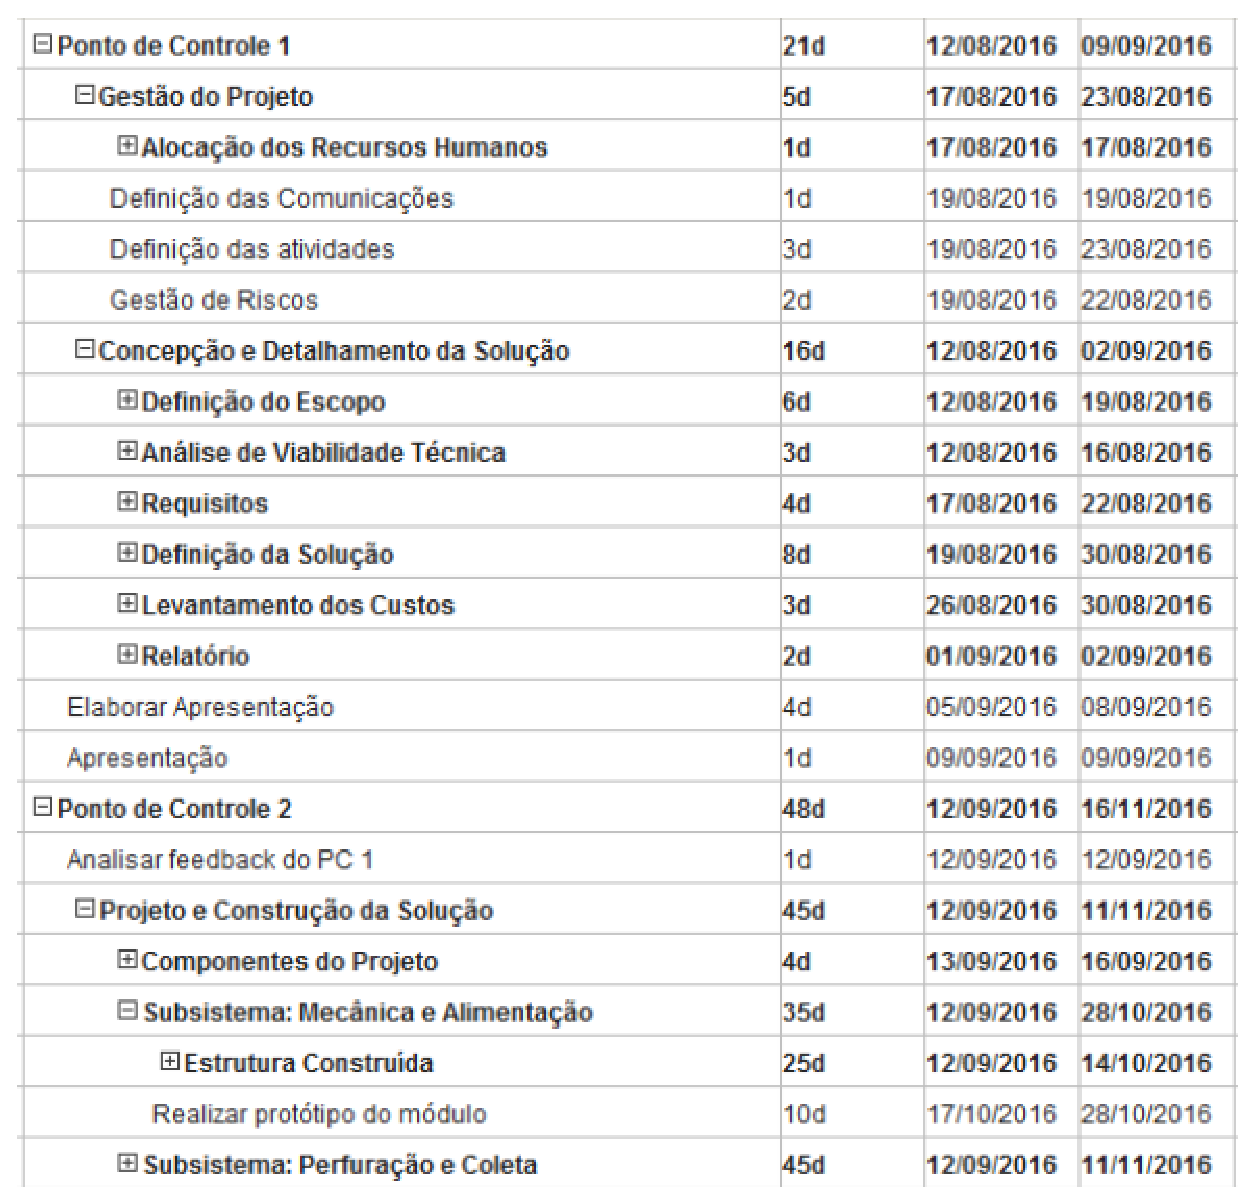
\includegraphics[width=\textwidth]{figuras/cronograma_simples_1.eps}
        \caption{Cronograma de Atividades simplificado (parte 1). Fonte: autores}
        \label{fig:cron_s1}
      \end{figure}

      \clearpage

      \begin{figure}[!htbp]
        \centering
        \includegraphics[width=\textwidth]{figuras/cronograma_simples_2.eps}
        \caption{Cronograma de Atividades simplificado (parte 2). Fonte: autores}
        \label{fig:cron_s2}
      \end{figure}

      \vfill
      \pagebreak


  \section{Riscos}
	\subsection{Objetivos}
	Este documento tem como finalidade estabelecer um processo de gerenciamento de riscos que podem vir a acontecer no projeto e a identificação dos mesmos pela equipe.

	\subsection{Descrição dos processos de gerenciamento de riscos}
	O Plano de Gerenciamento de Riscos contém seus processos definidos em quatro abordagens específicas segundo Max \cite{wideman1992project}. Sendo que todas as abordagens são necessárias pois elas se complementam para gerenciamento todas elas foram adotadas, sendo elas:
	
		\graphicspath{{figuras/}}
		\begin{figure}[h]
		\centering
		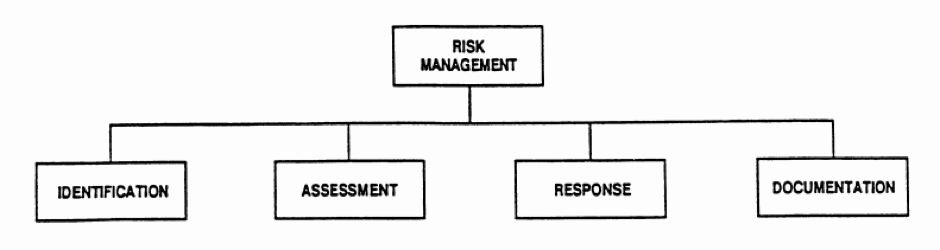
\includegraphics[scale=0.80]{EAP_Gerenciamento_de_Riscos.png}
		\caption{Etapas do plano de gerenciamento de riscos segundo Max \cite{wideman1992project}}
		\label{img:eap_gerenciamento_de_risco}
		\end{figure}
	
	\begin{itemize}
	 \item \textbf{Identificação}: Esta fase consiste em identificar todos os possíveis riscos que podem impactar de forma severa o sucesso do projeto. Os tipos de impacto podem variar dependendo de onde ele afeta no projeto e quais as probabilidades deles acontecerem. Combinações de riscos que juntos podem representar uma ameaça mais do que individualmente não podem ser ignorados.
	 \item \textbf{Avaliação}: Tendo identificado todo o alcance de riscos possíveis o próximo passo é os avaliar. O propósito é determinar os atributos do erro como o impacto, probabilidade e tipo de erro.
	\item \textbf{Resposta}: A parte de mitigação de riscos no projeto consiste em estabelecer uma estratégia de sistema apropriada, assim garantindo uma abordagem apropriada aos riscos caso eles venham a acontecer. Nesta etapa é descrito qual será a reação da equipe para tratar algum tipo de risco caso ele venha a acontecer.
	\item \textbf{Documentação}: Documento final e vital para o projeto que detalha todos os riscos, com suas características e quais serão as ações tomadas pela equipe de forma detalhada,caso cada risco apontado chegue a acontecer.
	\end{itemize}

	\subsection{EAR - Estrutura Analítica de Riscos para identificação dos riscos}
	O Project Management Institute (PMI), instituto que elaborou o Project Management Book of Knowledge (PMBoK) \cite{pmbok2012}, possui um template de estrutura analitica de riscos que possui as seguintes categorias e sub-divisões: 
	
	\graphicspath{{figuras/}}
	\begin{figure}[h!]
	\centering
	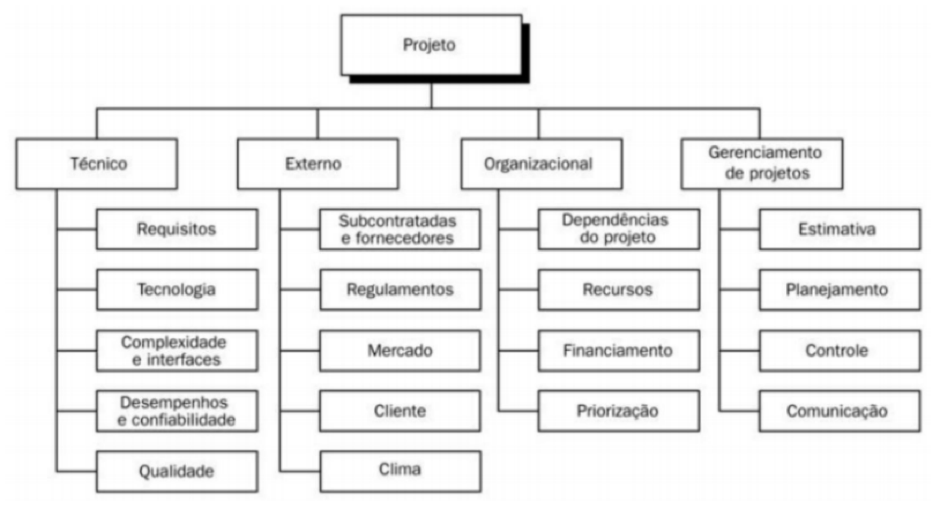
\includegraphics[scale=0.80]{classificacao_de_riscos.png}
	\caption{Classificação dos riscos na EAR segundo o PMI}
	\label{img:classificacao_de_riscos}
	\end{figure}
	
	\graphicspath{{figuras/}}
	\begin{figure}[h!]
	\centering
	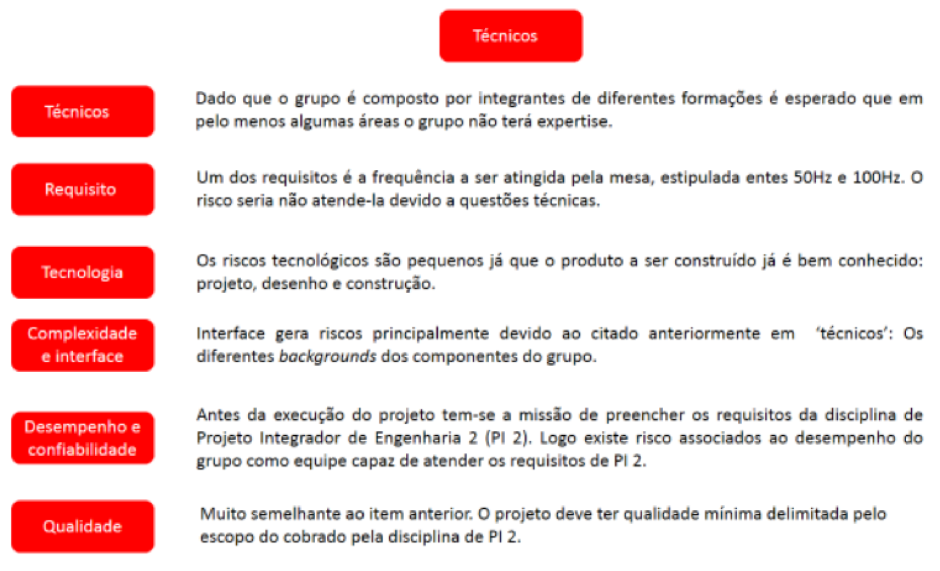
\includegraphics[scale=0.80]{analise_riscos_tecnicos.png}
	\caption{Análise em relação aos riscos técnicos}
	\label{img:analise_riscos_tecnicos}
	\end{figure}
	
	\graphicspath{{figuras/}}
	\begin{figure}[h!]
	\centering
	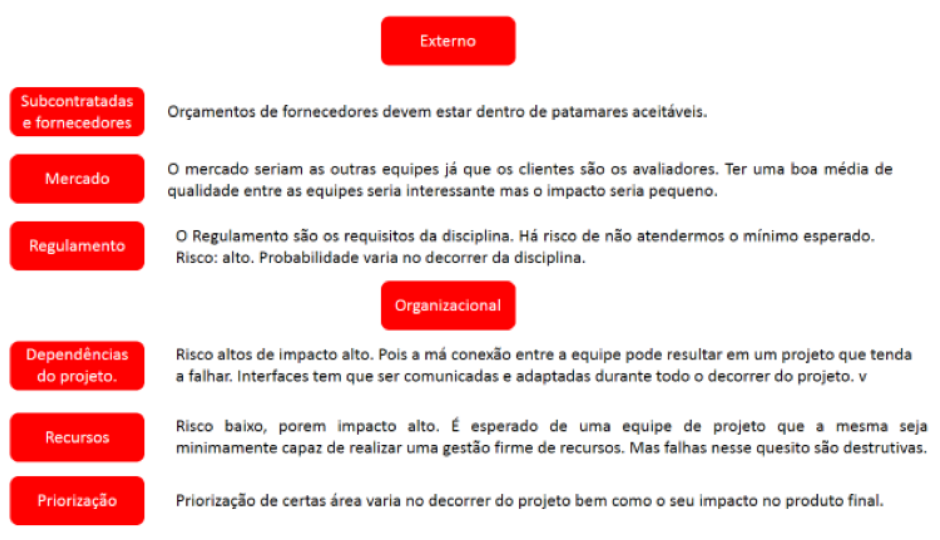
\includegraphics[scale=0.80]{analise_riscos_externos.png}
	\caption{Análise em relação aos riscos externos e organizacionais}
	\label{img:analise_riscos_externos}
	\end{figure}	
	
	\subsection{Qualificação dos Riscos}
	Os riscos identificados pelo grupo foram qualificados de acordo com sua probabilidade de ocorrência e o impacto resultante no projeto. O sistema de probabilidade e impactos foram classificados de acordo com a tabela padronizada do Gantter (ferramenta de gerenciamento de riscos adotada pela equipe).
	
	\begin{table}[h!]
\centering
\caption{Probabilidade dos Riscos}
\label{tabela_probabilidade_riscos}
\begin{tabular}{|ll|}
\hline
\multicolumn{1}{|l|}{\textbf{Nível}} & \textbf{Probabilidade} \\ \hline
Improvável                           & 0\% $\sim$ 20\%        \\
Remoto                               & 21\% $\sim$ 40\%       \\
Ocasional                            & 41\% $\sim$ 60\%       \\
Provável                             & 61\% $\sim$ 80\%       \\
Frequente                            & 81\% $\sim$ 100\%      \\ \hline
\end{tabular}
\end{table}	

\begin{table}[h!]
\centering
\caption{Severidade dos Riscos}
\label{tabela_severidade_de_riscos}
\begin{tabular}{|ll|}
\hline
\multicolumn{1}{|l|}{\textbf{Nível}} & \textbf{Descrição}                                                                                                                                                             \\ \hline
Negligível                           & Risco que não afeta a integridade do projeto de forma a comprometer o mesmo.                                                                                                   \\ \hline
Baixo                                & Possui pouco prejuízo ao desenvolvimento do projeto.                                                                                                                           \\ \hline
Moderado                             & \begin{tabular}[c]{@{}l@{}}Prejudica o desenvolvimento do projeto. Pode ser resolvido\\ em um curto período de tempo.\end{tabular}                                             \\ \hline
Significante                         & \begin{tabular}[c]{@{}l@{}}Prejudica o desenvolvimento do projeto. Gasta-se um tempo significativo\\ (semanas) para conseguir restituir a integridade do projeto.\end{tabular} \\ \hline
Catastrófico                         & Erro que previne o projeto de ser concluído.                                                                                                                                   \\ \hline
\end{tabular}
\end{table}
	
	\subsection{Prioridade dos Riscos}
	A prioridade dos riscos também foi feita de acordo com as opções já padronizadas da ferramenta “Gantter”, sendo elas:
	
	\begin{table}[h!]
\centering
\caption{Prioridade dos Riscos}
\label{tabela_prioridade_dos_riscos}
\begin{tabular}{|ll|}
\hline
\multicolumn{1}{|l|}{\textbf{Nível}} & \textbf{Descrição}                                                                                                                                                                                                                  \\ \hline
Sem Ação                             & O risco é tão pequeno ou irrelevante que nenhuma ação será tomada.                                                                                                                                                                  \\ \hline
Monitorar                            & \begin{tabular}[c]{@{}l@{}}O risco possui um certo grau de causar problemas, sendo \\ monitorado constantemente.\end{tabular}                                                                                                       \\ \hline
Tomar Ação                           & \begin{tabular}[c]{@{}l@{}}O risco possui uma boa probabilidade de causar problemas no projeto \\ e devem ser tomadas medidas de mitigação para que o mesmo não \\ aconteça ou reduza seu impacto.\end{tabular}                     \\ \hline
Ação Urgente                         & \begin{tabular}[c]{@{}l@{}}O risco possui uma boa probabilidade de causar muitos problemas no \\ projeto e devem ser tomadas medidas prioritárias de mitigação para que\\  o mesmo não aconteça ou reduza seu impacto.\end{tabular} \\ \hline
Interromper Projeto                  & \begin{tabular}[c]{@{}l@{}}O risco é tão significante que se interrompe o projeto até que seja \\ encontrada uma forma de contornar tal erro.\end{tabular}                                                                          \\ \hline
\end{tabular}
\end{table}	
	
	\subsection{Riscos Identificados}
	Os riscos identificados para o projeto estão listados na Tabela \ref{riscos_identificados}

\begin{table}[h!]
\centering
\caption{Riscos Identificados}
\label{riscos_identificados}
\begin{tabular}{|llll|}
\hline
\multicolumn{1}{|l|}{\textbf{Risco}}       & \multicolumn{1}{l|}{\textbf{Probabilidade}} & \multicolumn{1}{l|}{\textbf{Severidade}} & \textbf{Prioridade} \\ \hline
Trancamento de um integrante do grupo      & Remoto                                      & Moderada                                 & Monitorar           \\ \hline
Atraso nas entregas das atividades         & Provável                                    & Significante                             & Ação Urgente        \\ \hline
Desentendimento entre os membros da equipe & Ocasional                                   & Baixa                                    & Monitorar           \\ \hline
Atraso na entrega de um produto/serviço    & Ocasional                                   & Significante                             & Ação Urgente        \\ \hline
Problemas com a API                        & Remoto                                      & Catastrófica                             & Ação Urgente        \\ \hline
Vibração do motor                          & Remoto                                      & Baixa                                    & Monitorar           \\ \hline
Aquecimento dos componentes                & Remoto                                      & Moderada                                 & Monitorar           \\ \hline
Ergonomia do produto                       & Remoto                                      & Baixa                                    & Monitorar           \\ \hline
Custo inviável                             & Remoto                                      & Significante                             & Monitorar           \\ \hline
Atraso/falta dos integrantes nas reuniões  & Remoto                                      & Moderada                                 & Tomar Ação          \\ \hline
\end{tabular}
\end{table}

	\subsection{Ação de Resposta aos Riscos}
	As ações que foram definidas pelo time à serem tomadas para cada risco identificado se encontram na Tabela \ref{acoes_de_resposta}.

\begin{table}[!h]
\centering
\caption{Ações de Respostas aos Riscos}
\label{acoes_de_resposta}
\begin{tabular}{|ll|}
\hline
\multicolumn{1}{|l|}{\textbf{Risco}}       & \textbf{Resposta}                                                                                        \\ \hline
Trancamento de um integrante do grupo      & \begin{tabular}[c]{@{}l@{}}Redistribuir as atividades entre os \\ membros da mesma equipe\end{tabular}   \\ \hline
Atraso nas entregas das atividades         & \begin{tabular}[c]{@{}l@{}}Realinhar o cronograma e atuação do \\ responsável por tal grupo\end{tabular} \\ \hline
Desentendimento entre os membros da equipe & Alinhamento de idéias através dos líderes                                                                \\ \hline
Atraso na entrega de um produto/serviço    & \begin{tabular}[c]{@{}l@{}}Reunião dos líderes e tomada de ação no \\ setor com problemas\end{tabular}   \\ \hline
Problemas com a API                        & Procurar uma nova API                                                                                    \\ \hline
Vibração do motor                          & Procurar uma solução melhor                                                                              \\ \hline
Aquecimento dos componentes                & Replanejamento da estrutura                                                                              \\ \hline
Ergonomia do produto                       & Replanejamento da estrutura                                                                              \\ \hline
Custo inviável                             & Replanejamento dos componentes                                                                           \\ \hline
Atraso/falta dos integrantes nas reuniões  & \begin{tabular}[c]{@{}l@{}}Comunicação entre os representantes do \\ grupo com o indivíduo\end{tabular}  \\ \hline
\end{tabular}
\end{table}
	
	\subsection{Sistema de Controle de Mudanças de Riscos}
	O sistema serve justamente para alinhar a equipe sobre os riscos que o projeto pode vir a ter em seu decorrer e quais serão as ações que devem ser tomadas para cada tipo. A equipe deve estar consciente da probabilidade de cada risco encontrado a fim de controlar e manter o progresso do projeto em um meio que o risco possa sempre ser evitado.

	Cada risco não encontrado pelo grupo na fase de elaboração do projeto deverá ser documentado neste documento no futuro segundo os padrões adotados pela equipe e da ferramenta usada por ela para gerenciamento de riscos.
